\documentclass[border=5pt]{standalone}
\usepackage[T1]{fontenc}
\usepackage[utf8]{inputenc}
\usepackage{amsmath}
\usepackage{graphicx}
\usepackage{tikz}
\usetikzlibrary{positioning,arrows.meta,calc}
\begin{document}
\resizebox{150mm}{!}{%
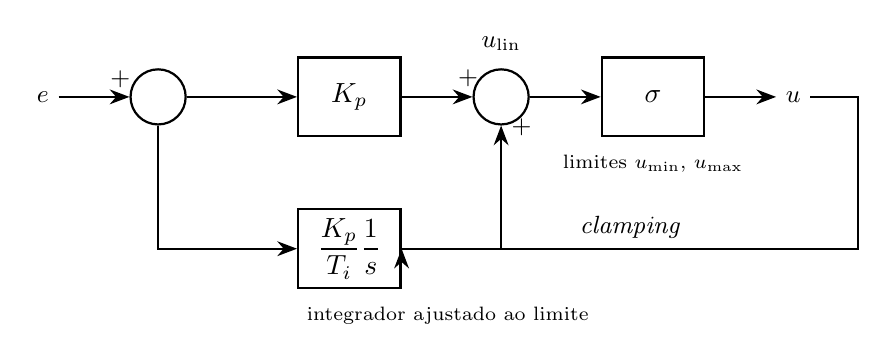
\begin{tikzpicture}[
  block/.style={draw=black, thick, minimum height=10mm, minimum width=13mm, inner sep=2pt},
  sum/.style={circle, draw=black, thick, minimum size=7mm, inner sep=0pt},
  sign/.style={font=\itshape\small},
  arr/.style={-{Stealth[length=2.5mm]}, thick},
  node distance=8mm and 9mm,
]
\node[sign] (e) {$e$};
\node[sum, right=of e] (s1) {};
\node[sign] at ($(s1.center)+(-4.8mm,2.2mm)$) {$+$};
% caminho P
\node[block, right=14mm of s1] (kp) {$K_p$};
% caminho I (abaixo)
\node[block, below=9mm of kp,
      align=center] (ki) {$\dfrac{K_p}{T_i}\dfrac{1}{s}$};
\node[sum, right=of kp] (soma2) {};
\node[sign] at ($(soma2.center)+(-4.2mm,2.4mm)$) {$+$};
\node[sign] at ($(soma2.center)+(2.6mm,-3.8mm)$) {$+$};
\node[sign, above=1mm of soma2] (ulin) {$u_{\mathrm{lin}}$};
\node[block, right=of soma2] (sat) {$\sigma$};
\node[font=\scriptsize, below=1mm of sat, align=center] {limites $u_{\min}$, $u_{\max}$};
\node[sign, right=of sat] (u) {$u$};

\draw[arr] (e) -- (s1);
\draw[arr] (s1) -- (kp);
\draw[arr] (s1) |- (ki);
\draw[arr] (kp) -- (soma2);
\draw[arr] (ki) -| (soma2);
\draw[arr] (soma2) -- (sat);
\draw[arr] (sat) -- (u);
% realimentacao de clamping: de u volta ao integrador
\draw[arr] (u.east) -- ++(6mm,0) |- ($(ki.east)+(0mm,0)$)
  node[pos=0.75, sign, above] {clamping} (ki.east);
\node[font=\scriptsize, align=center, anchor=north west] at ($(ki.south west)+(0mm,-1mm)$)
  {integrador ajustado ao limite};
\end{tikzpicture}%
}
\end{document}
